\documentclass[journal=jacsat,manuscript=article]{achemso}

\usepackage[version=3]
{mhchem} % Formula subscripts using \ce{}

\usepackage{listings}
\usepackage{minted}

\newcommand*\mycommand[1]{\texttt{\emph{#1}}}

%%%%%%%%%%%%%%%%%%%%%%%%%%%%%%%%%%%%%%%%%%%%%%%%%%%%%%%%%%%%%%%%%%%%%
%% Meta-data block
%% ---------------
%% Each author should be given as a separate \author command.
\author{Cas Wognum}
\affiliation{Valence Labs, Montréal, Québec, Canada}
\altaffiliation{Recursion Pharmaceuticals, Salt Lake City, UT, USA}
\author{Devany West}
\affiliation{Open Molecular Software Foundation, Davis CA, USA}
\author{Alexander Matthew Payne}
\affiliation{Computational and Systems Biology Program, Sloan Kettering Institute, Memorial Sloan Kettering Cancer Center, New York, NY, USA}
\altaffiliation{Tri-Institutional PhD Program in Chemical Biology, Memorial Sloan Kettering Cancer Center, New York, NY, USA}
\author{Jenke Scheen}
\affiliation{Open Molecular Software Foundation, Davis CA, USA}
\author{Josh Horton}
\affiliation{Open Molecular Software Foundation, Davis CA, USA}
\author{A whole bunch of participants}
\affiliation{Participants' author list: SI 1}
\author{A whole bunch of ASAP people}
\affiliation{ASAP' author list: SI 2}
\author{Hugo MacDermott-Opeskin}
\affiliation{Open Molecular Software Foundation, Davis CA, USA}
\email{*hugo.macdermott-opeskin@omsf.io}

%%%%%%%%%%%%%%%%%%%%%%%%%%%%%%%%%%%%%%%%%%%%%%%%%%%%%%%%%%%%%%%%%%%%%
%% The document title should be given as usual. Some journals require
%% a running title from the author: this should be supplied as an
%% optional argument to \title.
%%%%%%%%%%%%%%%%%%%%%%%%%%%%%%%%%%%%%%%%%%%%%%%%%%%%%%%%%%%%%%%%%%%%%
\title{A Computational Community Blind Challenge on Pan-Coronavirus Drug Discovery Data}

\begin{document}

%%%%%%%%%%%%%%%%%%%%%%%%%%%%%%%%%%%%%%%%%%%%%%%%%%%%%%%%%%%%%%%%%%%%%
%% The abstract environment will automatically gobble the contents
%% if an abstract is not used by the target journal.
%%%%%%%%%%%%%%%%%%%%%%%%%%%%%%%%%%%%%%%%%%%%%%%%%%%%%%%%%%%%%%%%%%%%%
\begin{abstract}
Computational blind challenges offer critical, real-world assessment opportunities to enable scientific progress as demonstrated by a breadth of breakthroughs over the last decade. We report the outcomes and key insights from an open science community blind challenge focused on antiviral drug discovery for coronaviruses using lead optimisation data from the ASAP Discovery consortium. This collaborative initiative invited global participants to develop and apply computational methods to predict the biochemical potency and crystallographic ligand poses of small molecules against a key coronavirus target - as well as multiple absorption, distribution and metabolism (ADMET) assay endpoints - using undisclosed experimental datasets as benchmarks. By evaluating submissions across multiple tasks and compounds, we established performance leaderboards and conducted meta-analyses to assess methodological strengths, common pitfalls, and areas for future improvement. We also highlight how use of next-generation benchmarking platforms such as Polaris enable best practices in blind challenge design and model evaluation to be embedded in the challenge infrastructure and provide a platform for community engagement.  This paper synthesizes the collective findings of the challenge, offering a high-level overview of the data, the evaluation framework, and the best-performing strategies. In doing so, it provides context and support for the accompanying papers authored by participants, which explore individual approaches in greater depth. Together, these contributions aim to accelerate drug discovery by advancing reproducible data-driven methods in an open, collaborative environment as well as exploring best practices and pitfalls in future blind challenge design and execution. 
\end{abstract}

%%%%%% MAKE THE WHOLE MANUSCRIPT DOUBLE COLUMN FOR EASIER FIGURE FORMATTING
% \twocolumn
%%%%%%%%%%%%%%%%%%%%%%%%%%%%%%%%%%%%%%%%%%%%%%%%%%%%%%%%%%%%%%%%%%%%%
%% INTRODUCTION
%%%%%%%%%%%%%%%%%%%%%%%%%%%%%%%%%%%%%%%%%%%%%%%%%%%%%%%%%%%%%%%%%%%%%
\section{Introduction}
%% DRUG DISCOVERY COMPCHEM DOESNT GET ENOUGH DATA FOR PROPER MODELS
Computational chemistry for drug discovery is often hindered by a persistent data shortage problem, particularly when it comes to high-quality, diverse, and openly accessible datasets that explore chemical space around target-specific chemical series in high detail. Predictive models such as those used in structure-based drug design, molecular docking, and machine learning rely heavily on large volumes of reliable experimental data to be effective. However, much of this data remains proprietary, fragmented or improperly reported, limiting model performance and reproducibility. Open science initiatives that share large amounts of data will be pivotal in order for these models to be developed effectively going forward. 
%% TO BUILD PROPER MODELS WE NEED PROPER BENCHMARKS AND CHALLENGES
Beside data availability, methods to compare models are required for building sustainable, translatable computational models. Community blind challenges provide a structured and unbiased framework for evaluating computational methods in drug discovery. Several notable community blind challenges have driven progress in computational drug discovery: 
The \textit{CACHE initiative}\cite{ackloo_al-awar_amaro_arrowsmith_azevedo_al._2022} evaluates hit-finding methods by experimentally testing predicted compounds in a fully open, prospective and standardized framework. The D3R Grand Challenges\cite{parks_gaieb_chiu_yang_shao_walters_jansen_mcgaughey_lewis_bembenek_et} benchmarked pose prediction and affinity ranking algorithms (e.g. free energy calculation methods) using small, focused blinded protein–ligand datasets. The Statistical Assessment of Modeling of Proteins and Ligands (SAMPL) series\cite{amezcua_setiadi_mobley_2024} involved testing of a wide variety of physical properties like partition coefficients, logD, pKa and ligand hydration free energies. Finally, the CASP competition\cite{andriy_kryshtafovych_schwede_topf_krzysztof_2019} challenges participants to predict protein structures \textit{a-priori}, with famous breakthroughs like AlphaFold2 transforming drug target modeling.\cite{jumper_evans_pritzel_green_figurnov_ronneberger_tunyasuvunakool_bates_žídek_2021} However, blind challenges have primarily been composed of datasets that were aggregated across drug discovery projects and in many cases across different drug discovery institutions. This presents a major gap in benchmarking the current state of the art of model performance on 'real-life' drug discovery problems that focus solely on a single project and span multiple modalities. 
%% ASAP DISCOVERY RAN AS OPEN SCIENCE AND APPROACHED PRECLINICAL CANDIDATE DISCLOSURE MILESTONE - PERFECT OPPORTUNITY
During the SARS-CoV-2 pandemic the COVID Moonshot consortium has demonstrated feasibility of developing a straight-to-generics Mpro inhibitor in record time using an open science approach. Building on this success, the ASAP Discovery Consortium  has been launched as an NIH AViDD center that leverages structure-enabled and artificial-intelligence approaches together with a global team to tackle structural biology, medicinal chemistry, biochemistry and (pre-)clinical trials for antiviral drug discovery. One of the main pillars of ASAP is the equitable licensing structure which ensures that global accessibility to antivirals is established. With ASAP's pan-coronavirus program (targeting SARS-CoV-2 and MERS-CoV Mpro) approaching a preclinical candidate disclosure in March 2025, a signficant portion of its drug discovery data was withheld to ensure a successful patent application within ASAP's equitable-access IP framework. This presented a unique opportunity to host a computational community blind challenge on this withheld dataset. 
%% PARTNERSHIP WITH POLARIS AND OPENADMET%%
Running a computational blind challenge requires significant community engagement, technical expertise and robust evaluation procedures. To this end, ASAP partnered with Valence Labs who have developed Polaris, an open platform to enable easy access to drug discovery datasets and benchmarks. Polaris provides robust challenge infrastructure, dataset hosting and expertise in best practices in model evaluation. Additionally, ASAP partnered with the team at OpenADMET, a new ARPA-H funded project under the Open Molecular Software Foundation (OMSF) focused around ADMET modeling. This challenge will from hereon be referred to as the ASAP-Polaris-OpenADMET Antiviral competition. 
%% QUICK DESCRIPTION OF WHAT DATA WAS IN THE CHALLENGE
The bulk of this dataset was composed of lead optimization data. The goal of this competition was to closely mirror the challenges that ASAP faced during its lead optimization campaign. To this end, three subchallenges were designed across three modalities common to drug discovery: 1) crystallographic ligand pose prediction, 2) biochemical potency prediction and 3) ADMET endpoint prediction (figure \ref{fgr:datasets_overview}).
\begin{figure}
    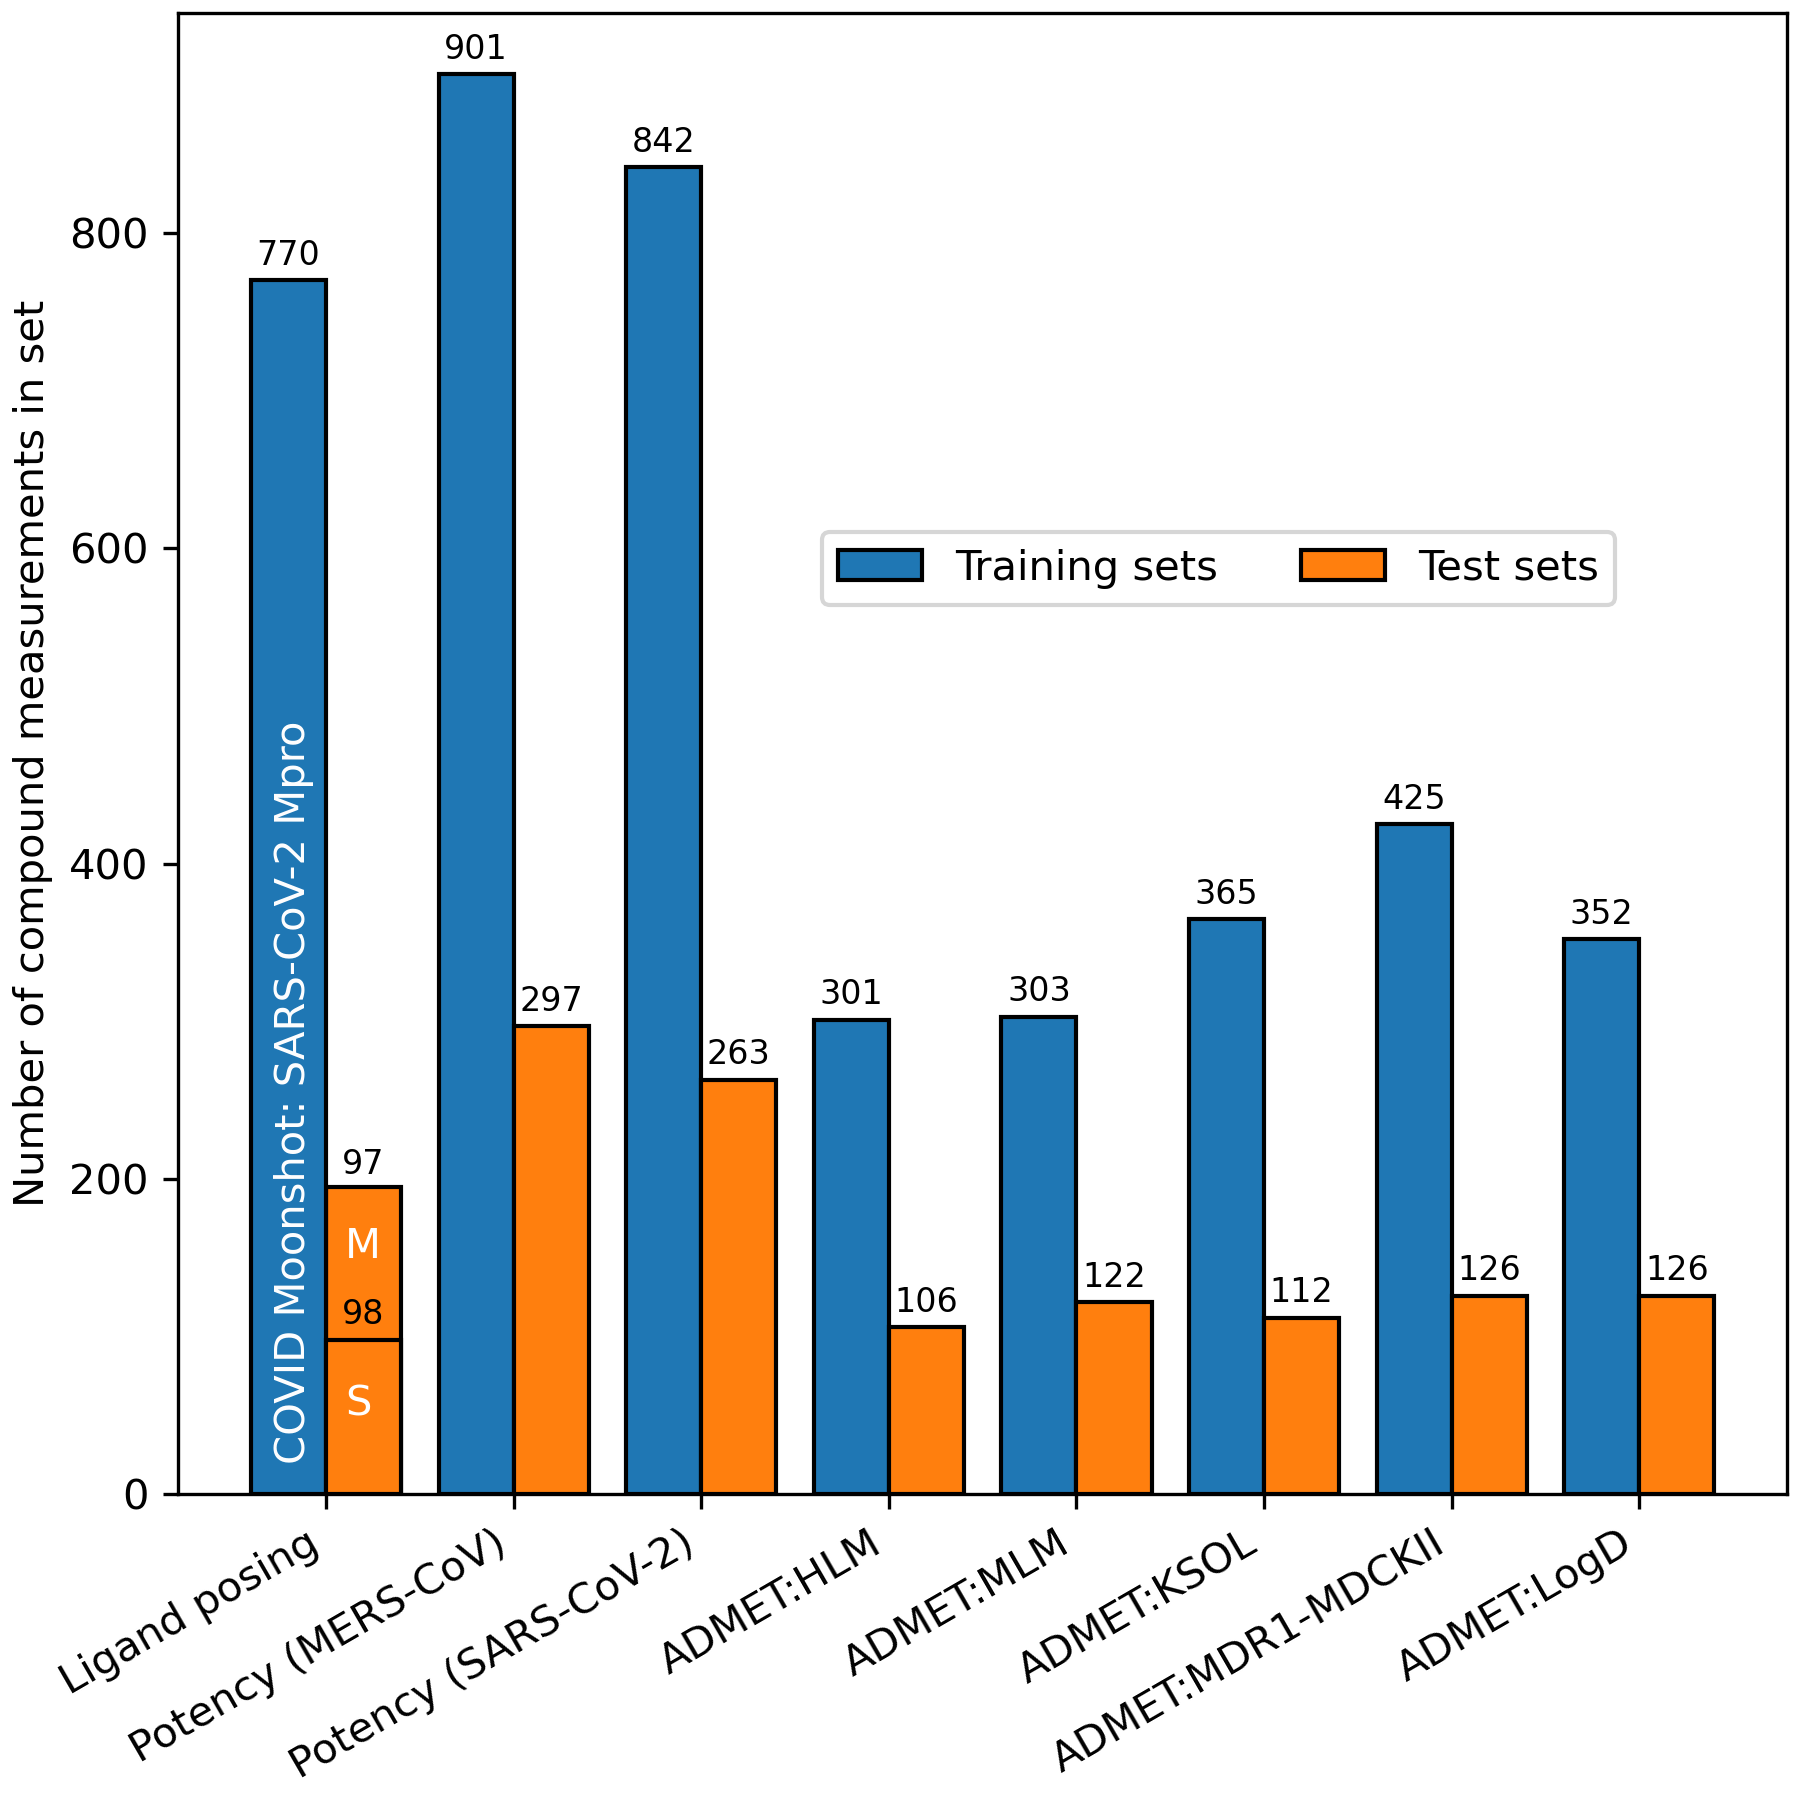
\includegraphics[scale=0.5]{01_figs_introduction/datasets_overview.png}
  \caption{Sizes of the datasets presented in this blind challenge across the different subchallenges. Training sets are shown as blue bars and test sets as orange bars with the total number of measurements annotated at the top of each bar. For the ligand posing subchallenge, \textbf{M} and \textbf{S} signify \textit{MERS-CoV Mpro} and \textit{SARS-CoV-2 Mpro} respectively. }
  \label{fgr:datasets_overview}
\end{figure}
%% MAIN OUTCOMES OF THE CHALLENGE
\begin{enumerate}
    \item this paper provides context and support for the accompanying papers authored by participants
    \item global response with lots of interest
    \item main learnings  
\end{enumerate}

%%%%%%%%%%%%%%%%%%%%%%%%%%%%%%%%%%%%%%%%%%%%%%%%%%%%%%%%%%%%%%%%%%%%%
%% COMMUNITY
%%%%%%%%%%%%%%%%%%%%%%%%%%%%%%%%%%%%%%%%%%%%%%%%%%%%%%%%%%%%%%%%%%%%%
\section{Platform \& Community}

 Polaris provides a python API based platform to enable easy access to drug discovery datasets and benchmarks. Relative to similar platforms such as Kaggle, Polaris includes dedicated support for modalities common in drug discovery, including small molecules, proteins and omics level data and acts as a single source of truth. Polaris' support for multiple drug discovery relevant modalities was critical for the multimodal nature of the challenge.  Additionally, Polaris is able to leverage significant expertise from their advisory board comprised of academic and industry experts around best practices for model evaluation and benchmarking. Open, real world dataset benchmarks hosted on Polaris can help build trust in computational methods for drug discovery, by enabling direct comparison and reducing the potential for XXXX. Additionally, Polaris allowed us to leverage a community already interested in open science and machine learning for drug discovery. 


- timeline, specifically all the things we did (walk-in sessions, intermediate leaderboards etc) and timing with ACS disclosure


\begin{figure}
    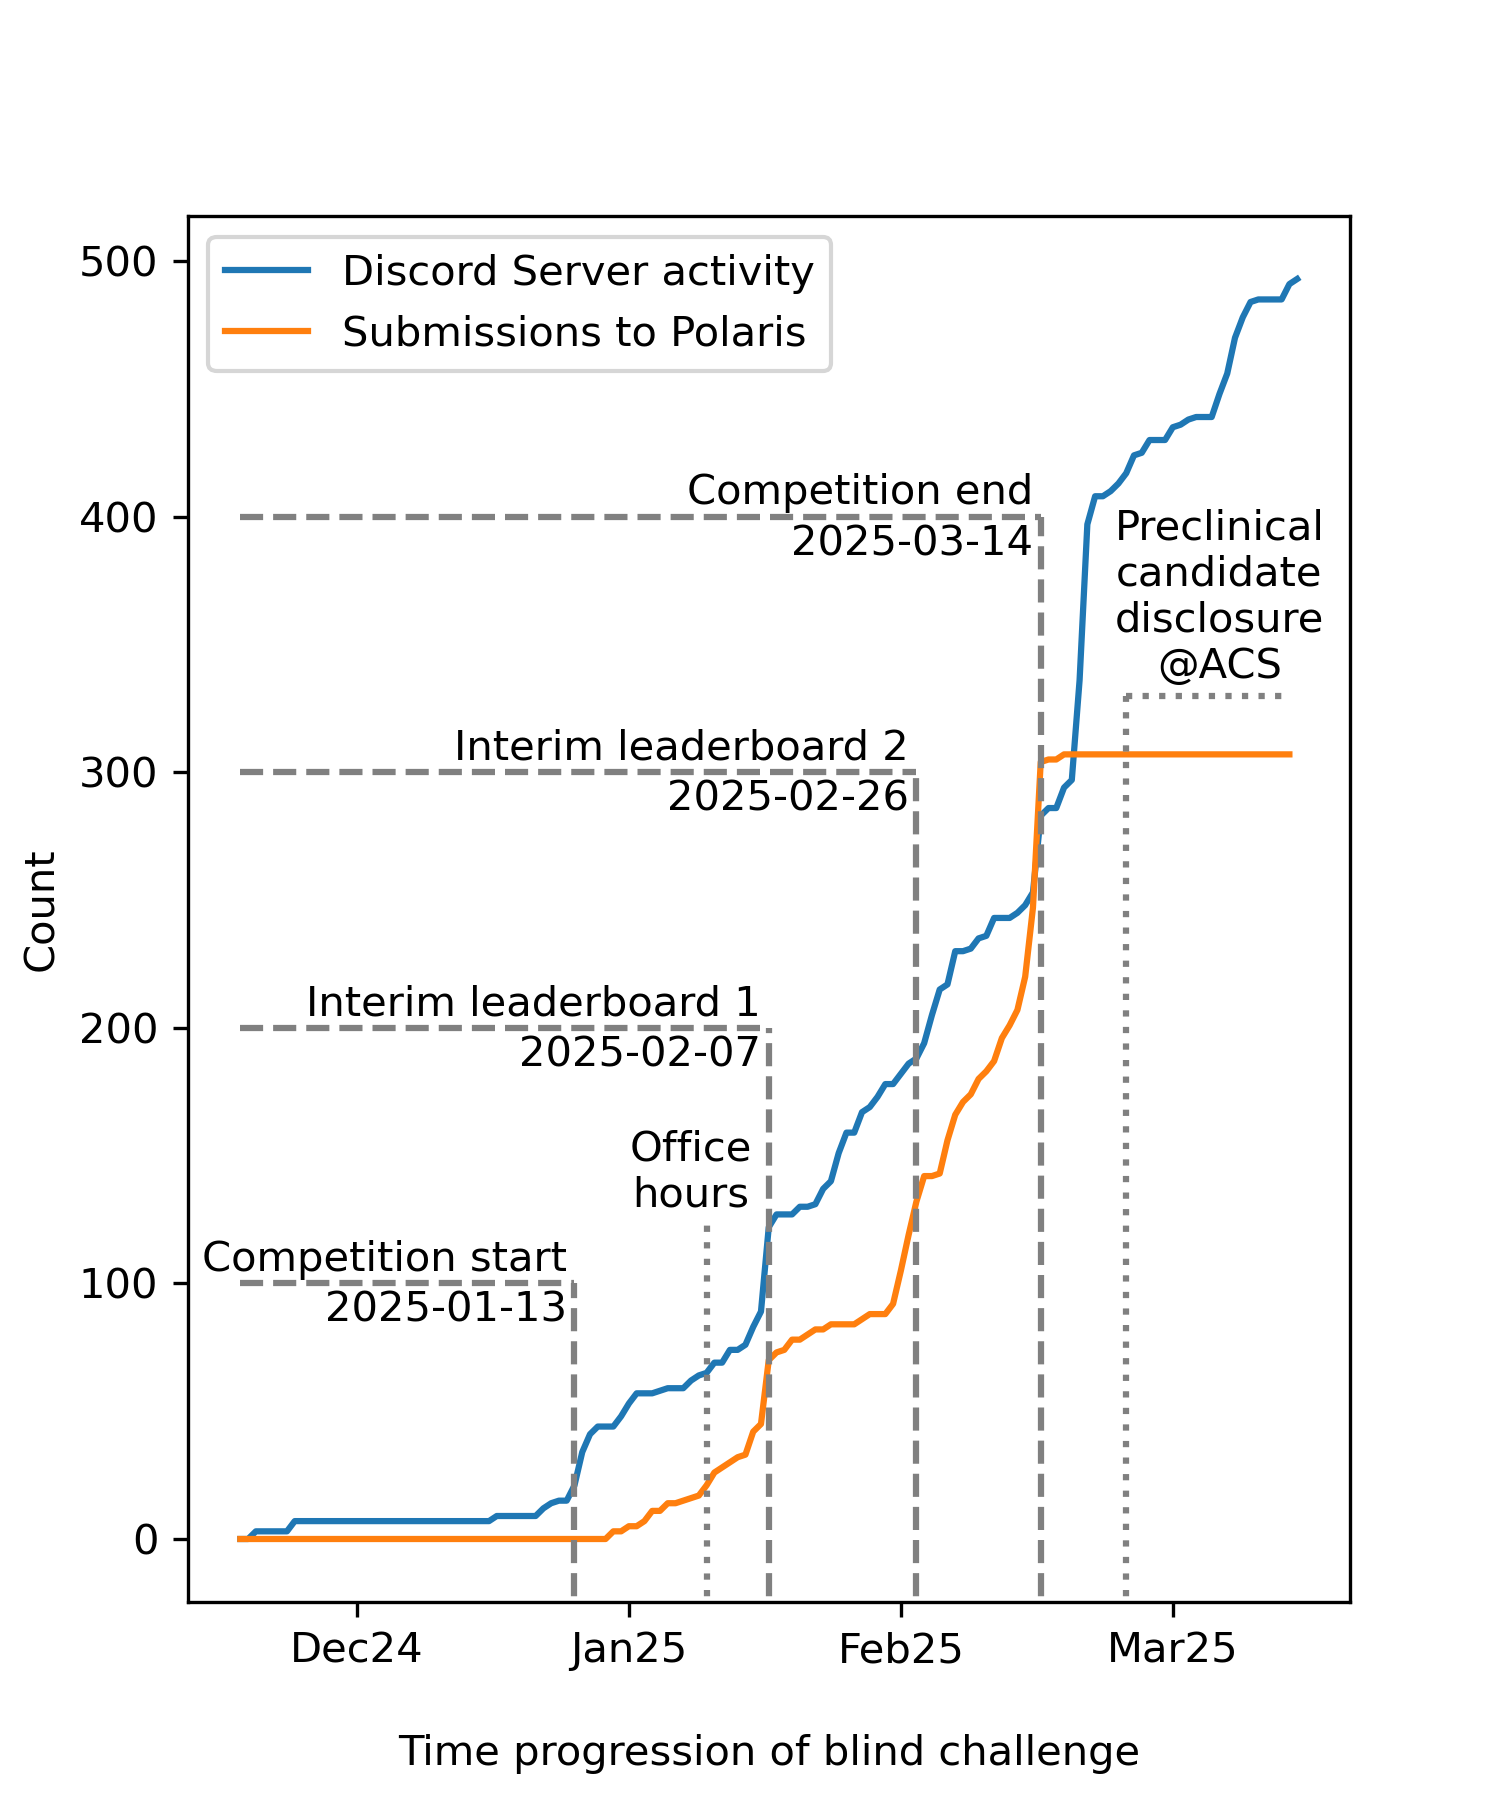
\includegraphics[scale=0.6]{02_figs_community/community_progression_lineplots.png}
  \caption{Community engagement for the blind challenge across its runtime with several milestones annotated with corresponding dates. Shown are the number of messages sent by participants over the Discord server in blue and the number of predictions submitted by participants to the Polaris platform in orange. Dotted lines indicate the virtual office hours that were hosted on 2025-01-30 and 2025-01-31 and the preclinical candidate disclosure at ACS on 2025-03-25; after this date all test set data was published.}
  \label{fgr:timeline_engagement}
\end{figure}

\begin{figure}
    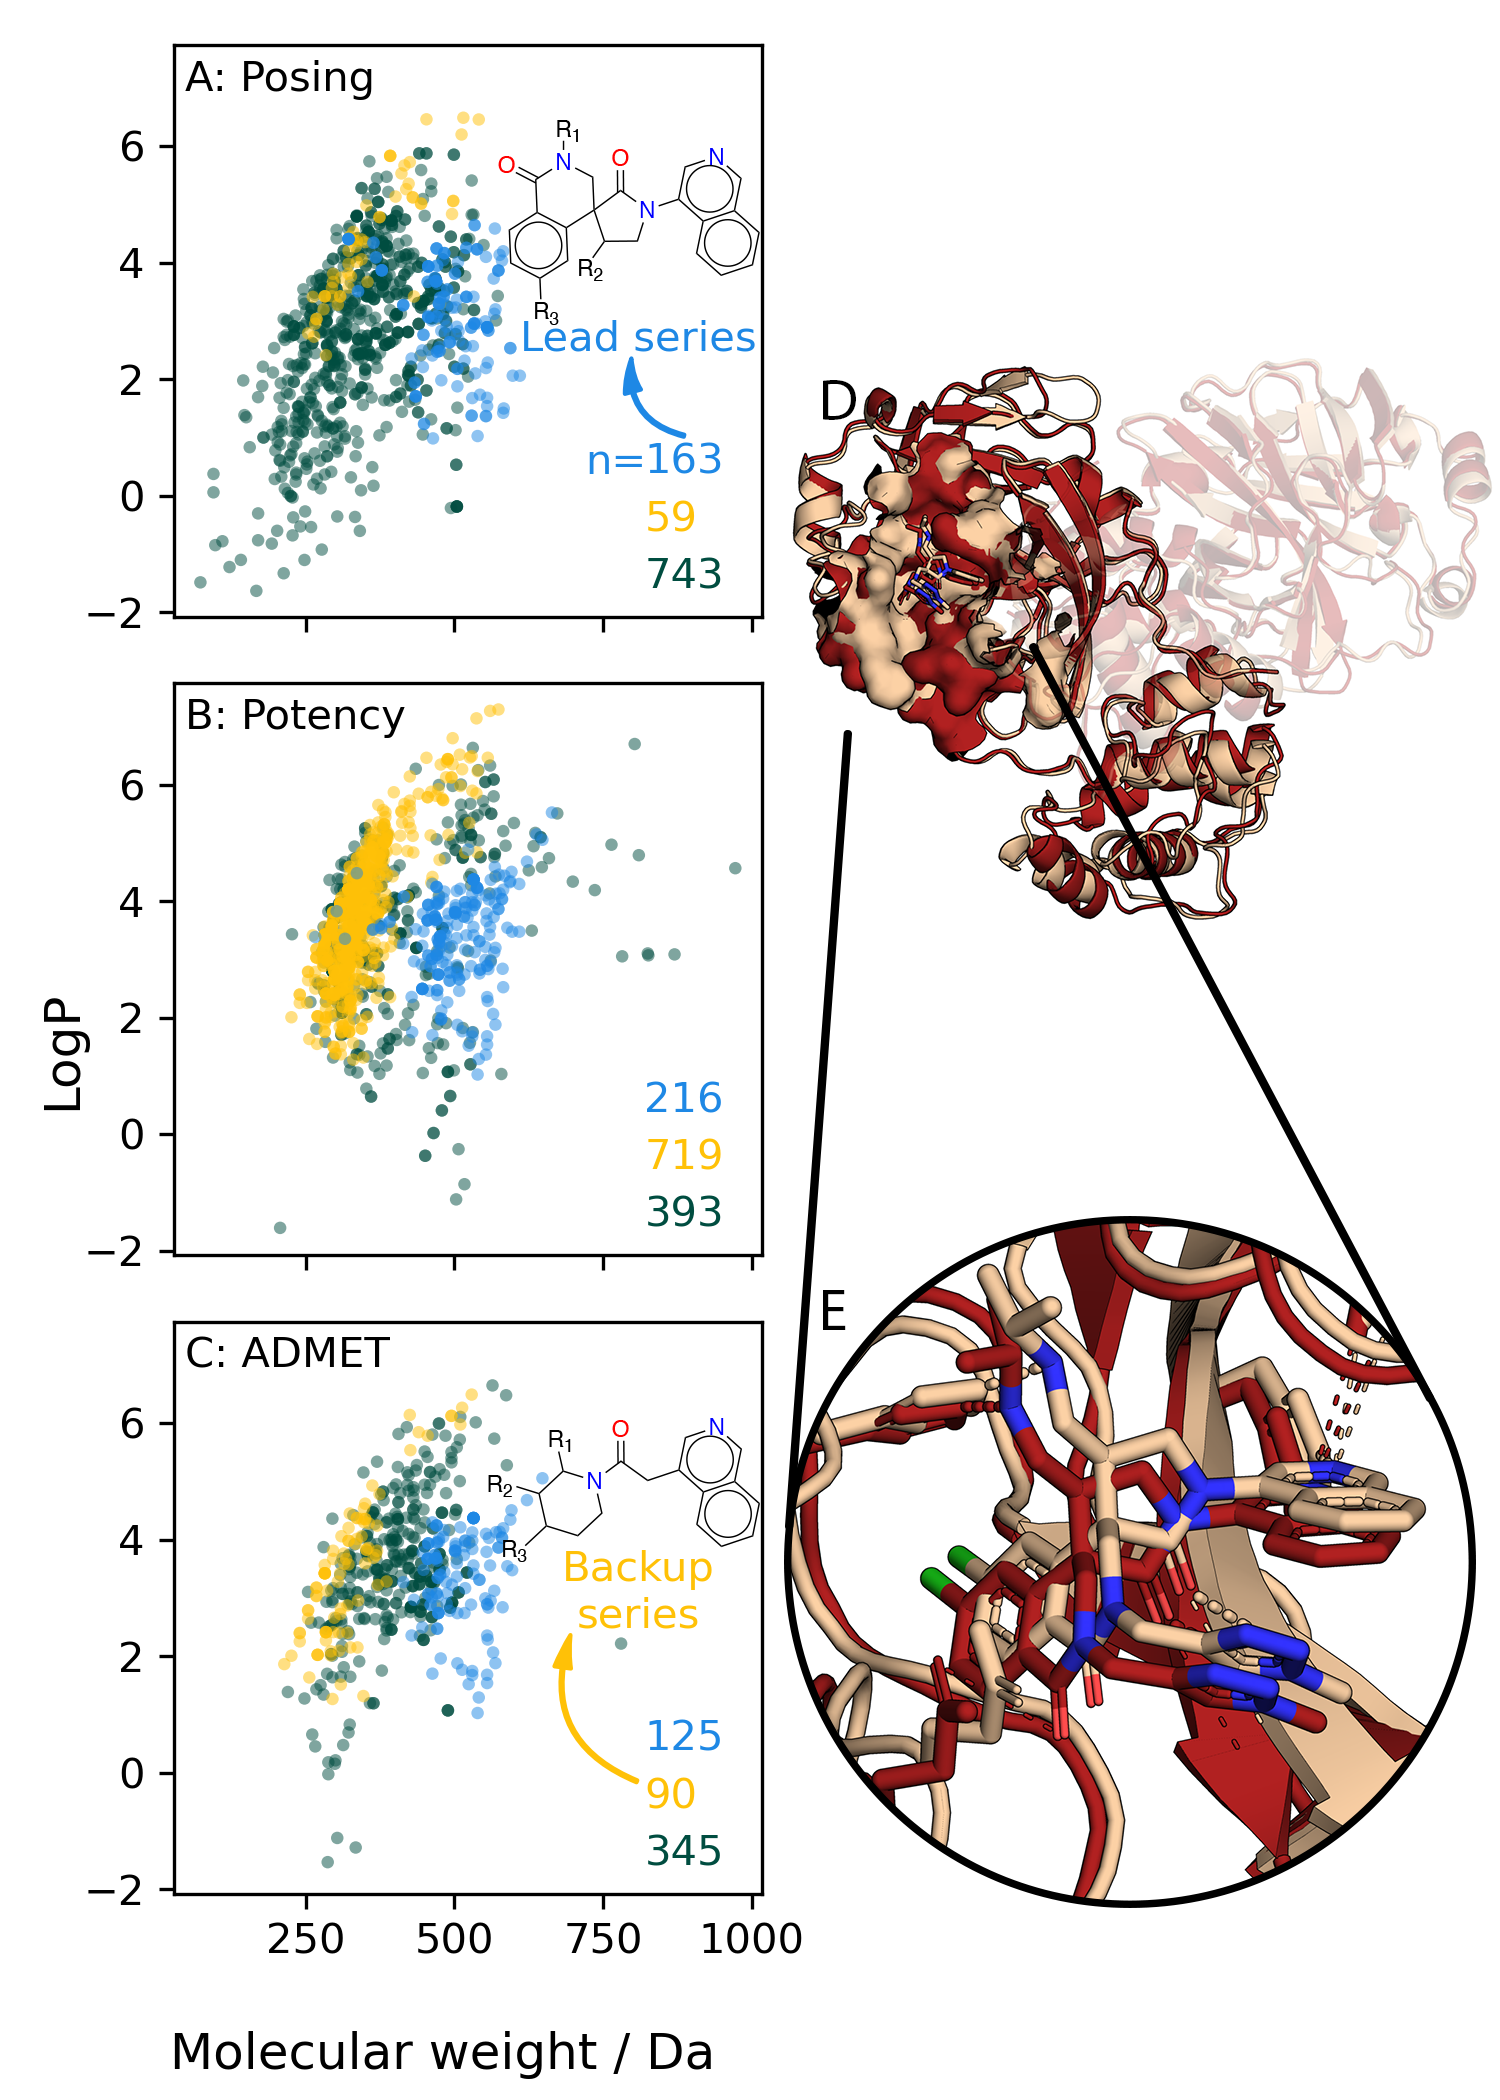
\includegraphics[scale=0.9]{03_figs_data_preparation/subchallenge_physprops_with_scaffolds.png}
  \caption{Subchallenge compounds span across multiple chemical series. }
  \label{fgr:physprops_scaffolds}
\end{figure}

%%%%%%%%%%%%%%%%%%%%%%%%%%%%%%%%%%%%%%%%%%%%%%%%%%%%%%%%%%%%%%%%%%%%%
%% DATA PREPARATION AND EVALUATION
%%%%%%%%%%%%%%%%%%%%%%%%%%%%%%%%%%%%%%%%%%%%%%%%%%%%%%%%%%%%%%%%%%%%%
\section{Data preparation \& evaluation of models}

Data was collated from ASAP Discovery’s pan-coronavirus main-protease (Mpro) inhibitor program (spanning both SARS-CoV-2 Mpro and MERS-CoV Mpro), which at the time of challenge initiation had successfully reached preclinical candidate nomination. Available data spanned three main modalities, in-vitro biochemical potency measurements, ADMET and structural biology (X-ray crystallography) across the two protein targets. 

As part of its pandemic preparedness mission ASAP has pursued an open-science policy in conjunction with an IP policy designed to ensure equitable and affordable global access to any derived therapeutics, while protecting ASAP from predatory competitive practices. This is achieved through phased open science in the early stages of drug discovery, followed by time limited confidentiality in later stages of lead optimisation and “minimally defensive patenting” for candidate molecules. Practical implications for the challenge were that molecules previously disclosed as part of our open-science efforts and those sufficiently congeneric to molecules claimed in a minimal patent defensive patent filed but not yet disclosed (the situation at the time of the challenge) could not be included in the challenge data.

The data collated for this challenge represents a uniquely focused blind challenge on a narrow chemical space taken from the progression of a real discovery program. This is in contrast to other benchmarking efforts and available public datasets that either sample broad areas of chemical space, contain an agglomeration of multiple data sources or attempt to simulate lead-opt-like progression algorithmically. The lead-opt-like nature of the potency and ADME datasets can be seen in the available dynamic ranges across the two modalities (See figure XX).  with primary density in areas considered acceptable for human therapeutics.  Additionally, due to early structural enablement of SARS-CoV-2 and later enablement of  MERS-CoV Mpro, the challenge contains a wealth of structural data rarely available in concert with detailed potency and ADME measurements.

In summary, the challenge presented herein represents a unique opportunity to benchmark computational methods on real-world drug discovery data. Both the focused coverage of chemical space and the density of data across different modalities is unique to this challenge and should present a realistic and informative benchmark for participants modelling efforts. Experimental conditions used to generate the challenge data and the structure of the challenge are detailed below.


\subsection{Reference data collection}

Mpro inhibition was measured via a direct in-vitro dose-response biochemical assay, using a fluorescent Mpro substrate. Experiments were performed primarily at the Weizmann Institute of Science. Technical differences between the assays for SARS-CoV-2 Mpro and MERS Mpro are explored in their respective protocols available online (here and here respectively) . Following data collection half maximal inhibitory concentrations (IC50s) were determined via fits to dose response curves.  The fitting procedure differed between SARS-CoV-2 Mpro and MERS Mpro due to differences in binding kinetics between the two proteins, both of which are homodimeric but differ in their association constants. SARS-CoV-2 Mpro used a traditional fit to a four parameter logistic function. For MERS Mpro, the weakly bound dimer can undergo ligand-induced dimerisation and an alternative curve fitting procedure used to account for the resulting low concentration activation. Challenge data used pIC50s (log10 IC50) as calculated from the raw IC50 values.

Crystal structures were expressed and purified by Centre for Medicines Discovery at the University of Oxford for SARS-CoV-2 Mpro and  MERS-CoV Mpro. Crystal constructs were created and soaked with compounds and analyzed at the X-ray beamline at Diamond Light Source according to the two protocols outlined for SARS-CoV-2 Mpro and MERS-CoV Mpro respectively. 

ADMET data was collected on an ADMET panel from the bioassay contract research organisation Bienta that was configured specifically for the Mpro program’s goals as defined in ASAP’s Target Candidate Profile for its pan-coronavirus Mpro program. This consisted of five primary endpoints: Mouse Liver Microsomal stability (MLM https://dx.doi.org/10.17504/protocols.io.5qpvokdb9l4o/v1), Human Liver Microsomal stability (HLM https://dx.doi.org/10.17504/protocols.io.5qpvokdb9l4o/v1), Kinetic Solubility (KSOL https://dx.doi.org/10.17504/protocols.io.j8nlk8y41l5r/v1), LogD as a measure of lipophilicity (https://dx.doi.org/10.17504/protocols.io.e6nvw14kdlmk/v1) and a cell permeability assay (Perm) in p-glycoprotein expressing Madin-Darby canine kidney cells (MDR1-MDCKII cells). https://dx.doi.org/10.17504/protocols.io.n2bvjne6ngk5/v1).  For the cell permeability assay the apical to basolateral apparent permeability was used as the primary endpoint.

\subsection{ML-ready dataset preparation}

Data was collated from ASAP’s CDD vault (research informatics database platform that aggregates assay outcomes on a molecule level).
Data was split into a training set that was released to participants and a blinded test set that participants were evaluated on. A 75:25 train:test split was selected for the ADMET and potency prediction challenges, while for the pose prediction challenge, data from the COVID Moonshot (also solved by X-ray crystallography at Diamond Light Source) was used as the training set totaling 770 structures for SARS-CoV-2 Mpro only, while the test set comprised 98 SARS-CoV-2 Mpro structures and 97 MERS-CoV Mpro structures from the ASAP Discovery Consortium.  

For the ADMET and potency subchallenges we used a temporal split of the data to create a challenge more  representative of real-world drug discovery, where molecules must be evaluated prospectively. However, this had to be balanced against minimization of leakage between endpoints which could jeopardise competition integrity. This was particularly challenging for the ADMET subchallenge in which several endpoints have 
limited amounts of data. 

To balance these competing concerns, the following procedure was followed to split the data for the ADMET and potency subchallenges.  XXXX

Following splitting, data was cleaned to be ML-ready. Compounds marked as below or above assay detectable range with a ChEMBL style modifier (\textless=; \textgreater=) were removed. Duplicates molecules were removed, with some missed (see lessons learned). Where a molecule had data recorded for an endpoint more than once, the most recent data collection was selected. The final ML-ready datasets for ADMET and potency were organised as a multi-task matrix and uploaded to the Polaris platform. We also made the dataset with out of range datapoints and some additional endpoint-specific assay data available for the participants in case they wanted to leverage the additional negative data in their models.  



\subsection{Running the challenge on the Polaris platform \& engaging the community}

An example of how participants were expected to submit their predictions to the Polaris platform is shown in Listing XXX. This provides significant operational advantages relative to modes of running other challenges, which include large amounts of manual data handling. A consistent pythonic API also allows participants to co-locate their modeling efforts with submission to the challenge infrastructure e.g in a Jupyter notebook.

\setminted{baselinestretch=0.5} % decreases vertical spacing between lines
\begin{minted}{python}
import polaris as po

# load the competition data from the Polaris platform and split it
competition = po.load_competition("asap-discovery/antiviral-potency-2025")
train, test = competition.get_train_test_split()

# make predictions
y_pred = my_participant_model(test)

# submit predictions to the Polaris platform
competition.submit_predictions(
    predictions=y_pred,
    prediction_name="my-predictions",
    prediction_owner="participant_name",
    report_url="https://www.my_report.com",
)
\end{minted}

To enable participants to easily use the Polaris challenge infrastructure, we provided participants example notebooks with simulated baselines to demonstrate how to submit to each of the sub-challenges. 

Several technical challenges presented themselves for the modalities available in the ASAP challenge. In particular, evaluation of ligand-pose challenge proved complicated in way XXXX.


\subsection{Engaging the community}

Engaging with the scientific community and attracting high quality participants across academia and industry is critical to running an impactful blind challenge. Polaris has built significant momentum around both their platform and disseminating best practices, and have used a Discord server for community engagement. For the running of the challenge, we created a specific channel  that participants used prior, during and after the challenge for scientific and technical discussion, with the challenge responsible for significant growth in overall engagement on the Discord (figure \ref{fgr:timeline_engagement}). 

Additionally, we provided participants an opportunity to engage with experimentalists from ASAP and challenge organisers through two open office hours, where participants could enquire about assay parameters, conditions and analysis. We also conducted extensive social media campaigns to advertise both the office hours and challenge as a whole and organised a post-challenge symposium for top-performing participants to share their methodologies. 


\subsection{Evaluation procedure}    

Fair and robust evaluation of predictions is critical to the success of a blind challenge. Evaluation of computation predictions for chemical matter in drug discovery is evolving, with several recent papers outlining best practice in this area, and highlighting that robust evaluation is critical to trust and adoption of \textit{in-silico} methods. With this in mind, we attempted to come up with a rigorous evaluation procedure that would fairly evaluate participant's submissions while remaining easily interpretable to outside participants.

Evaluation procedures and metrics were chosen for each sub-challenge based on the data distributions and appropriate treatment for the data modality. For each subchallenge, multiple metrics were reported, with one metric chosen for primary ranking. Where a subchallenge is comprised of multiple endpoints (SARS-CoV-2 Mpro pIC50 and MERS-CoV Mpro pIC50 for potency, MLM, HLM, KSOL, LogD and Perm for ADMET) the macro averaged primary metric was used for ranking. For the potency and ADMET subchallenges the Mean Absolute Error (MAE), Mean Squared Error (MSE), Pearson's $R$, Spearman's $\rho$ and $R^2$ were reported. For the posing subchallenge, the success rate (number of poses with a ligand heavy atom RMSD below a threshold) at a threshold of 2Å was reported.

For the potency subchallenge, the pIC50s span a range of XX to XX (IC50s XX to XX, see figure \ref{fgr:XXX}). Mean absolute error (MAE) was chosen as an appropriate flexible continuous metric for potency evaluation. Ranking of compounds by potency is often viewed as at least as important as absolute potency prediction. To this end we also conducted analyses  with kendall's Tau.

For the ADMET subchallenge, endpoints span a wide range with significant outliers. To alleviate the impact of outliers on the evaluation, endpoints that were not already in a base 10 logarithmic scale were transformed to a base 10 logarithmic scale prior to evaluation. As some endpoints 

We also provided baselines for each of the challenge modalities, meant to represent. 



%%%%%%%%%%%%%%%%%%%%%%%%%%%%%%%%%%%%%%%%%%%%%%%%%%%%%%%%%%%%%%%%%%%%%
%% OUTCOMES
%%%%%%%%%%%%%%%%%%%%%%%%%%%%%%%%%%%%%%%%%%%%%%%%%%%%%%%%%%%%%%%%%%%%%
\section{Challenge Outcomes}
  
- ADMET
observations:
normalized mae by dynamic range to allow us to compare between admet endpoints
based on mae it looks like ksol is easy to predict but ranking is very poor; dynamic range too small for this assay to use mae as meaningful descriptor
talk about distributions fig and why we chose to log everything
ranking is more useful - based on this it looks like logd and permeability were easiest to predict, then hlm and mlm were doable.
why is ksol so hard to predict? does anyone do well on this? point to some papers
describe top entries and what they did well on
were there any entries that dropped the ball on any assays which caused them to end up lower on the leaderboard?



\begin{figure}
    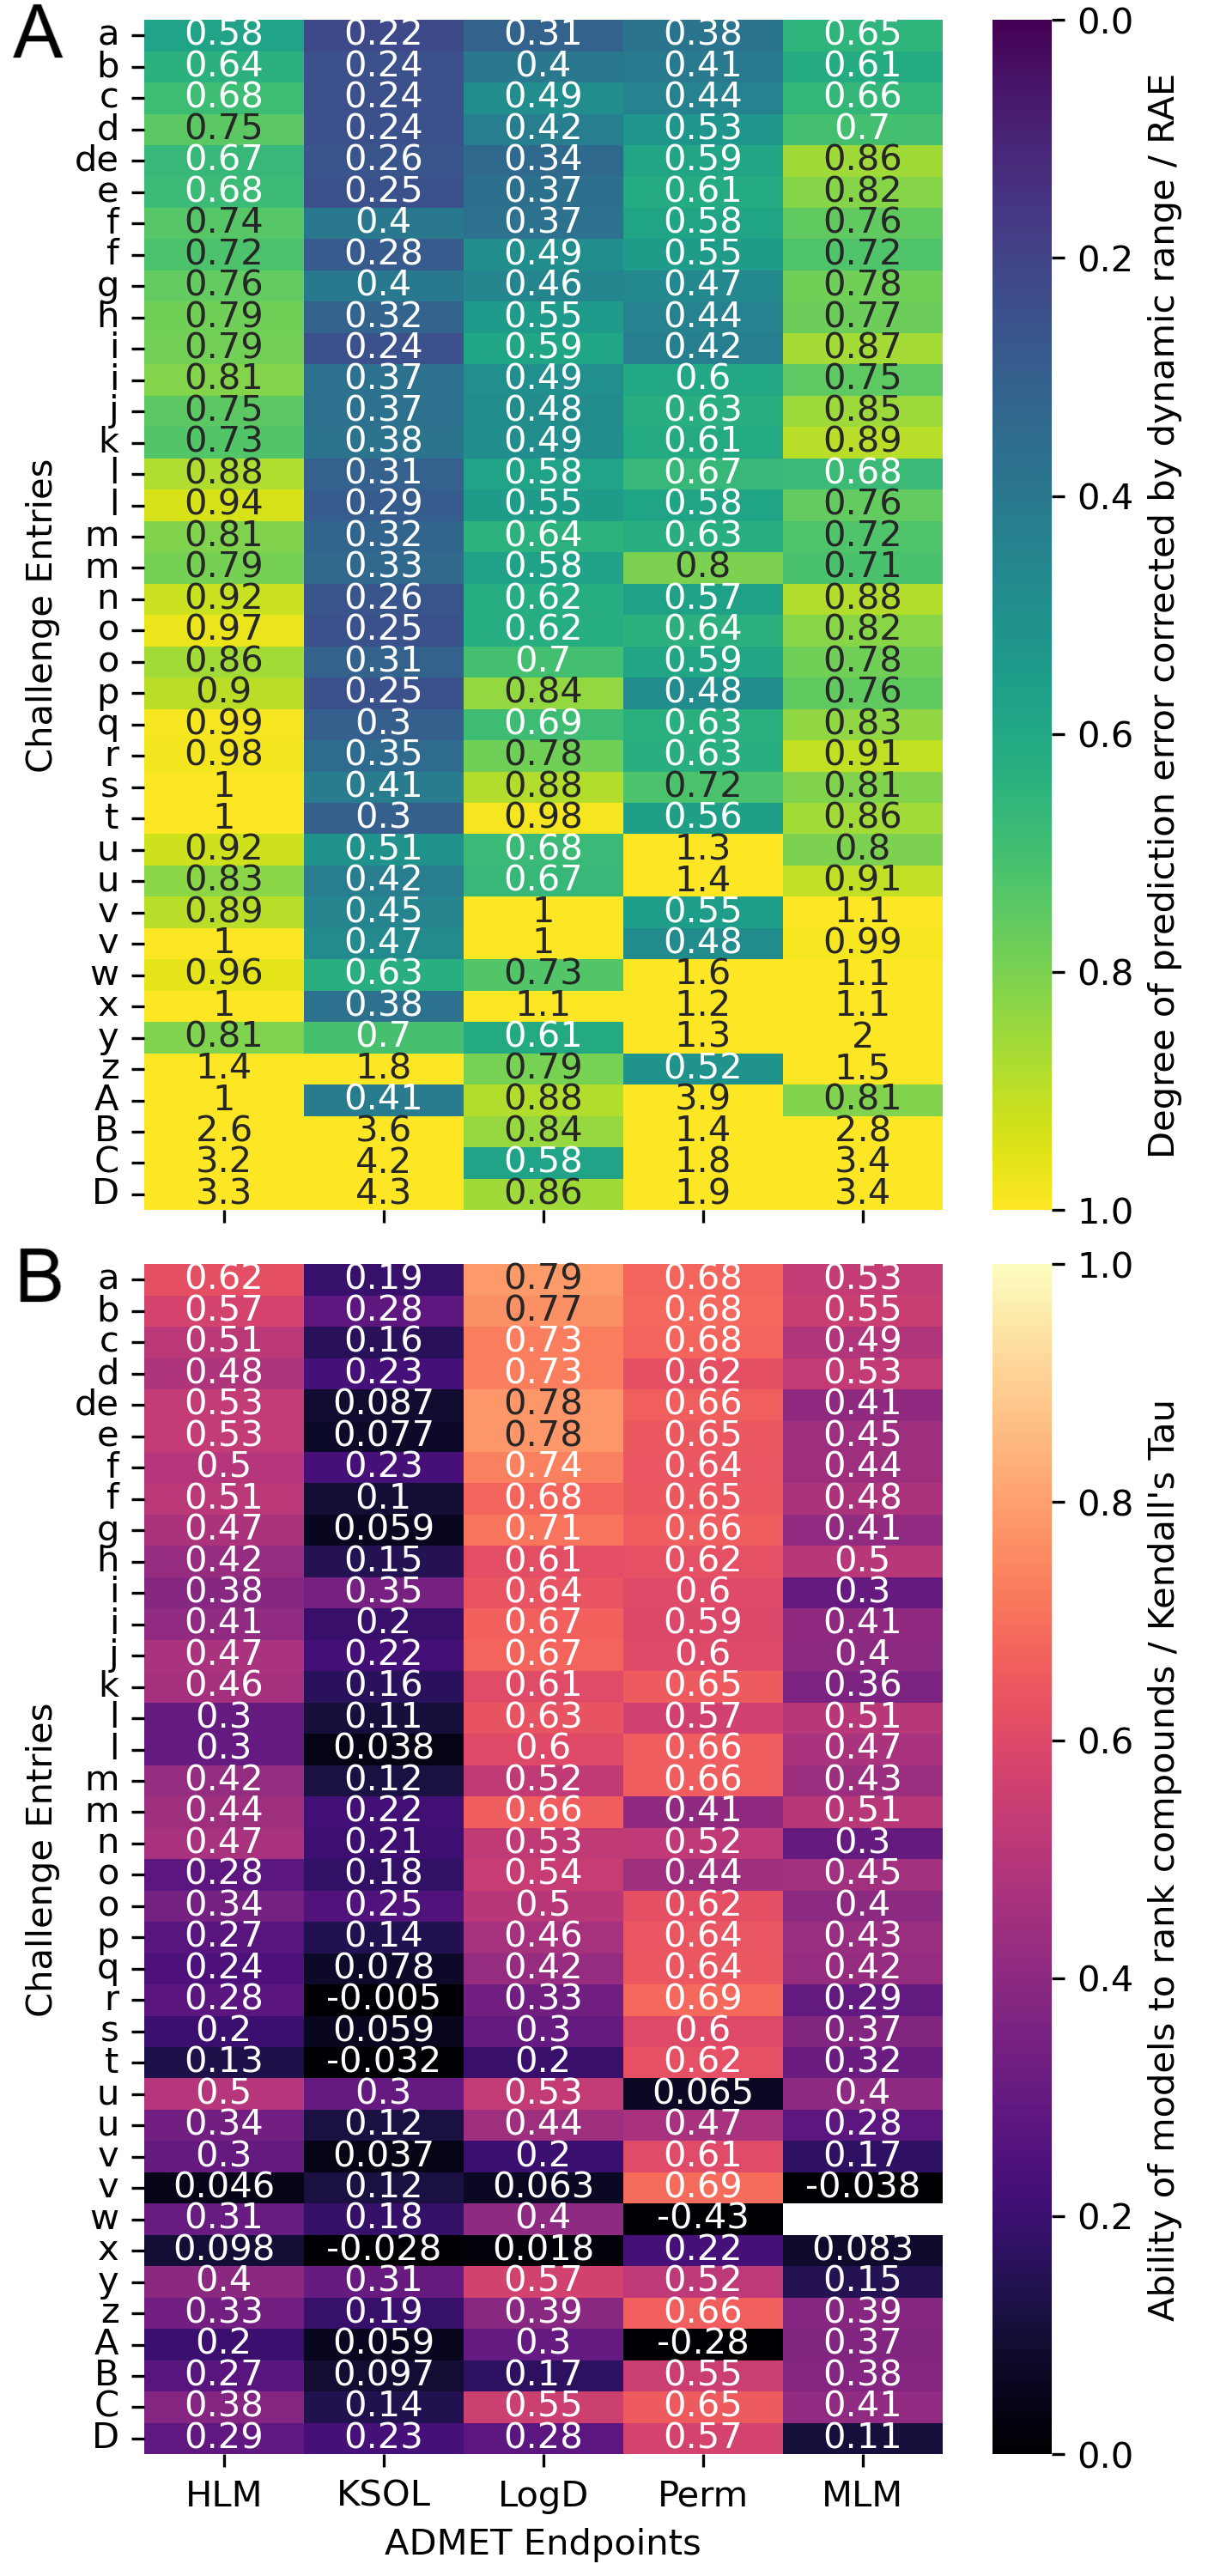
\includegraphics[scale=0.6]{04_figs_leaderboards/heatmaps.png}
  \caption{Participants' models performed poorly on kinetic solubility predictions but strongly on stability, permeability and lipophilicity. The empty cell at entry \textit{w} MLM consisted of constant predicted values thus no ranking coefficient was calculated.}
  \label{fgr:heatmaps_admet}
\end{figure}

- Poses
observations:
many outliers, only top performers had very few
generally more outliers for mers
median RMSD higher for mers than for sars2
one consistent sars2 outlier - our fault bc chain B
some entries posed into the wrong chain (j, m, q) - some user-side eval would have been useful here
cofolding methods dominated this subchallenge
physics-based docking methods were a mixed bag, overall reference-informed docking did best - mention baseline method
baseline method with uninformed docking did poorly - pose prediction in leadopt is probably better with other methods, but can still be useful for active/inactive separation
overall, >80 percent success rate is very impressive, would have been useful for mers at the time. is likely 'enough' for lead opt, but hard to say
\begin{figure}
    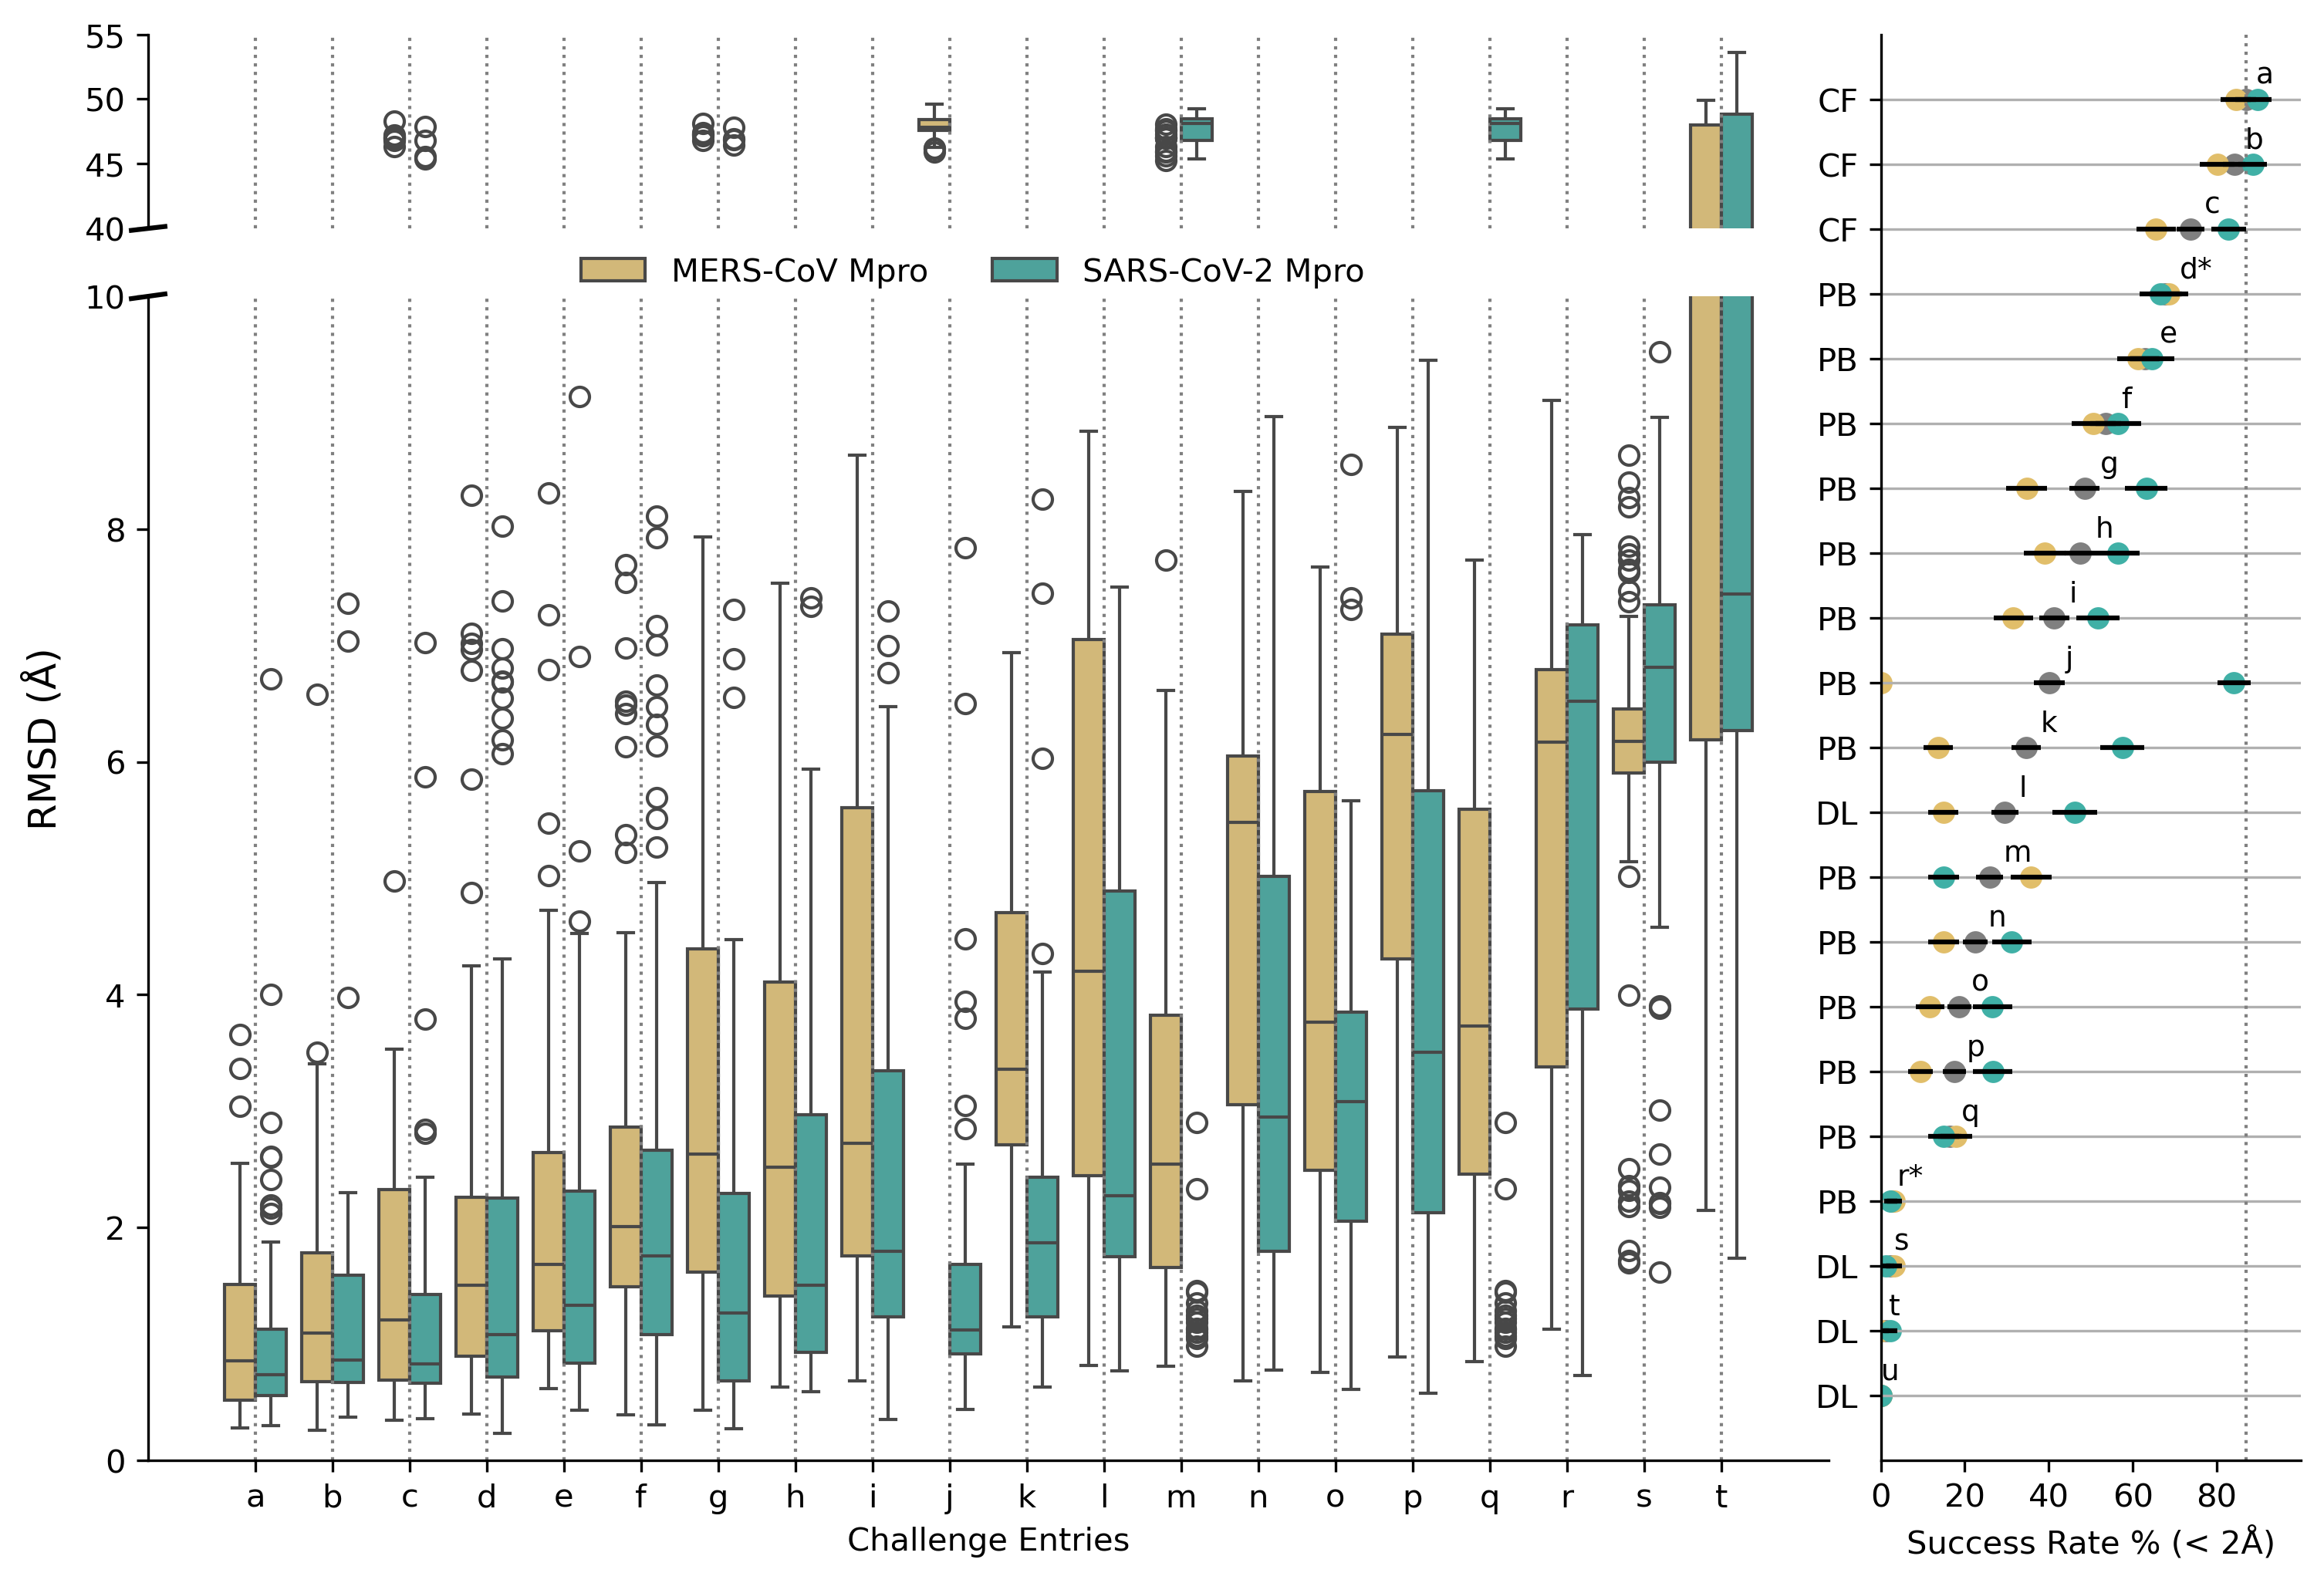
\includegraphics[scale=0.15
    ]{04_figs_leaderboards/pose_comp.png}
  \caption{Participants' generally performed better on the SARS-CoV-2 pose predictions with higher success rates, ligands predicted with an RMSD \textless2Å, and lower median RMSD predictions apart from one entry, \textit{m,} which shows the reverse prediction accuracy. Prediction RMSD distributions are shown for each entry split by the MERS-CoV and SARS-CoV-2 Mpro targets (left) with one entry removed u as the full distribution lies in the axis break. The success rate of each entry is shown (right) for the overall submission (grey) and the two targets separately to further highlight the difference in performance across the targets. The overall success rate was used to determine the final ranking of the submissions.}
  \label{fgr:poses_leaderboard}
\end{figure}
%%%%%%%%%%%%%%%%%%%%%%%%%%%%%%%%%%%%%%%%%%%%%%%%%%%%%%%%%%%%%%%%%%%%%
%% LEARNINGS
%%%%%%%%%%%%%%%%%%%%%%%%%%%%%%%%%%%%%%%%%%%%%%%%%%%%%%%%%%%%%%%%%%%%%
\section{Challenge Key Learnings}
[essentially a conclusions section]


things we messed up:
define categories to talk about:

communication/PR


polaris side:
no user-side eval



- lessons learned


\subsection{The future of blind challenges}

We believe that blind challenges are the best way to robustly assess models and drive forward computational methods in drug discovery. This is validated by step-change improvements in model performance after community investment in blind challenges both in related fields such as computer vision (XX and XX), natural language processing (XX and XX) and abstract reasoning (XX and XX), and in those relevant to drug discovery such as computational structure prediction (CASP). Infastructure like Polaris XXX. 

















%%%%%%%%%%%%%%%%%%%%%%%%%%%%%%%%%%%%%%%%%%%%%%%%%%%%%%%%%%%%%%%%%%%%%
%% The "Acknowledgement" section can be given in all manuscript
%% classes.  This should be given within the "acknowledgement"
%% environment, which will make the correct section or running title.
%%%%%%%%%%%%%%%%%%%%%%%%%%%%%%%%%%%%%%%%%%%%%%%%%%%%%%%%%%%%%%%%%%%%%
\begin{acknowledgement}

Please use ``The authors thank \ldots'' rather than ``The
authors would like to thank \ldots''.

\end{acknowledgement}

%%%%%%%%%%%%%%%%%%%%%%%%%%%%%%%%%%%%%%%%%%%%%%%%%%%%%%%%%%%%%%%%%%%%%
%% The same is true for Supporting Information, which should use the
%% suppinfo environment.
%%%%%%%%%%%%%%%%%%%%%%%%%%%%%%%%%%%%%%%%%%%%%%%%%%%%%%%%%%%%%%%%%%%%%
\begin{suppinfo}

This will usually read something like: ``Experimental procedures and
characterization data for all new compounds. The class will
automatically add a sentence pointing to the information on-line:

\end{suppinfo}

%%%%%%%%%%%%%%%%%%%%%%%%%%%%%%%%%%%%%%%%%%%%%%%%%%%%%%%%%%%%%%%%%%%%%
%% The appropriate \bibliography command should be placed here.
%% Notice that the class file automatically sets \bibliographystyle
%% and also names the section correctly.
%%%%%%%%%%%%%%%%%%%%%%%%%%%%%%%%%%%%%%%%%%%%%%%%%%%%%%%%%%%%%%%%%%%%%
\bibliography{references}

\end{document}